
\documentclass[11pt,a4paper]{article}
\usepackage{amsmath,amssymb,graphicx}
\usepackage{geometry}
\geometry{margin=2.5cm}
\title{Experimental Protocols for UQCMF Tests}
\author{Prepared for ISGAC2026}
\date{\today}
\begin{document}
\maketitle

\section*{Overview}
This document presents three categories of feasible experiments for the Unified Quantum Cosmic--Mind Framework (UQCMF): Laboratory, Field, and Statistical tests.

\section{Laboratory Tests}
\subsection{Quantum Measurement Coupled with Human Decisions}
\textbf{Goal:} Detect deviations from standard quantum predictions when measurement settings are chosen by humans.
\textbf{Protocol:}
\begin{enumerate}
  \item Set up a photon entanglement source and polarisation measurement stations.
  \item Let human participants select measurement angles in real time.
  \item Record coincidence counts and compare with Bell inequality limits.
\end{enumerate}
\textbf{Equipment:} entangled photon source, polarisers, photon counters, computer.
\begin{figure}[h]
    \centering
    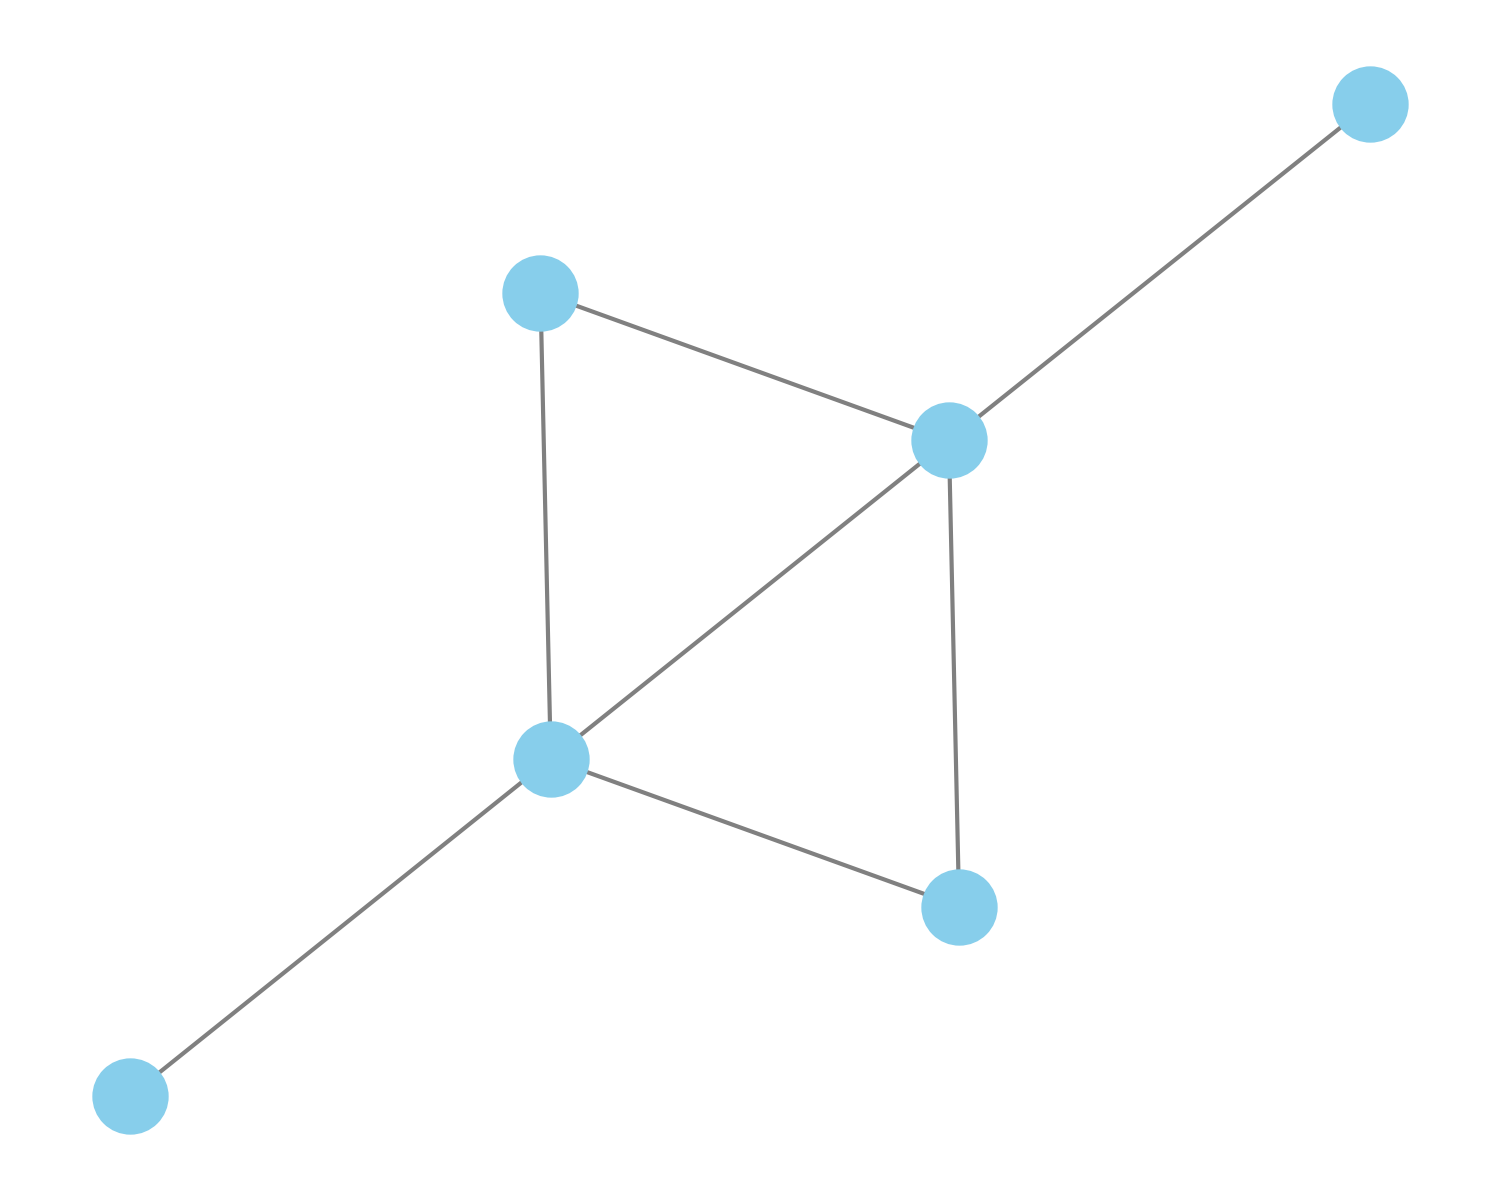
\includegraphics[width=0.75\textwidth]{figures/lab1_schematic.png}
    \caption{Schematic for quantum decision experiment.}
\end{figure}

\subsection{Brainwave Simulation on Sensitive Oscillators}
\textbf{Goal:} Detect potential physical influence of brainwave patterns.
\textbf{Protocol:}
\begin{enumerate}
 \item Record EEG from participants.
 \item Feed filtered signal into a micro-interferometer or piezoelectric sensor.
 \item Analyse vibration/phase shift statistics.
\end{enumerate}
\textbf{Equipment:} EEG headset, micro-interferometer/piezo sensor, DAQ unit.
\begin{figure}[h]
    \centering
    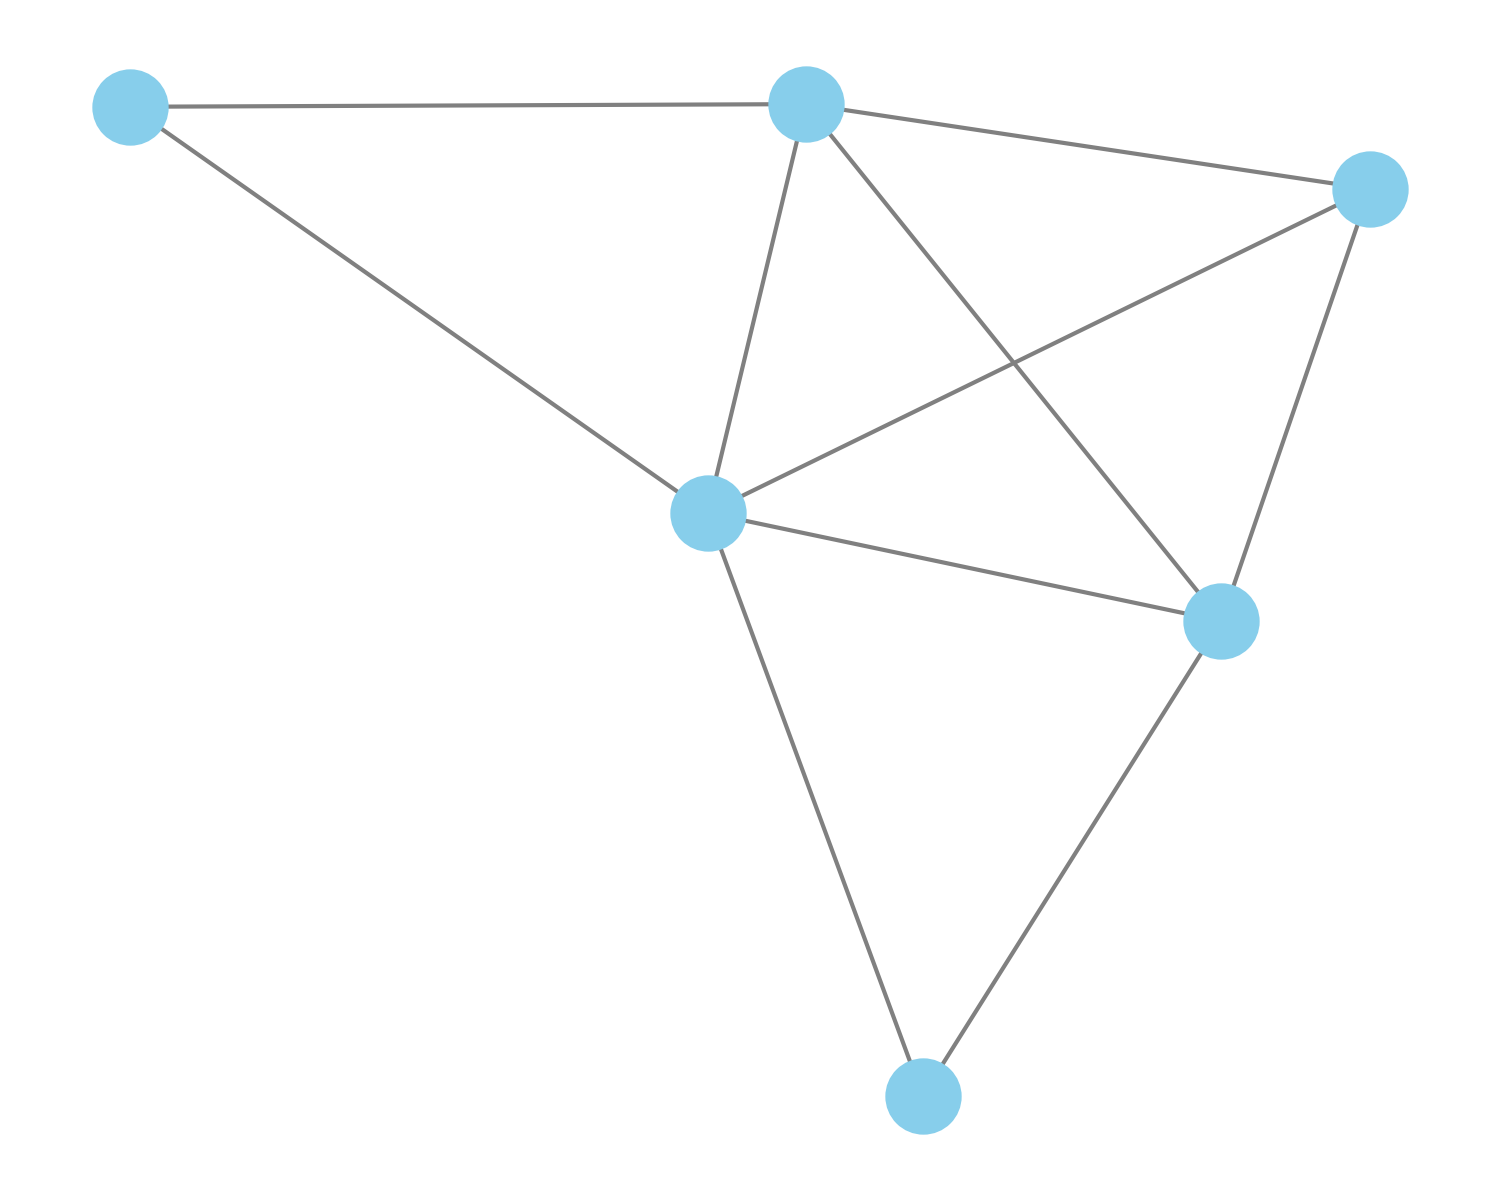
\includegraphics[width=0.75\textwidth]{figures/lab2_schematic.png}
    \caption{Brainwave-to-oscillator coupling schematic.}
\end{figure}

\section{Field Tests}
\subsection{Mental Response to Cosmic Events}
\textbf{Goal:} Identify EEG changes correlated with astrophysical events (e.g., GRBs, gravitational waves).
\textbf{Protocol:}
\begin{enumerate}
 \item Schedule EEG recording sessions overlapping predicted/known cosmic events.
 \item Tag event times from space/ground observatories.
 \item Compare pre-event and post-event EEG statistics.
\end{enumerate}
\textbf{Equipment:} EEG system, access to astrophysical event timing.
\begin{figure}[h]
    \centering
    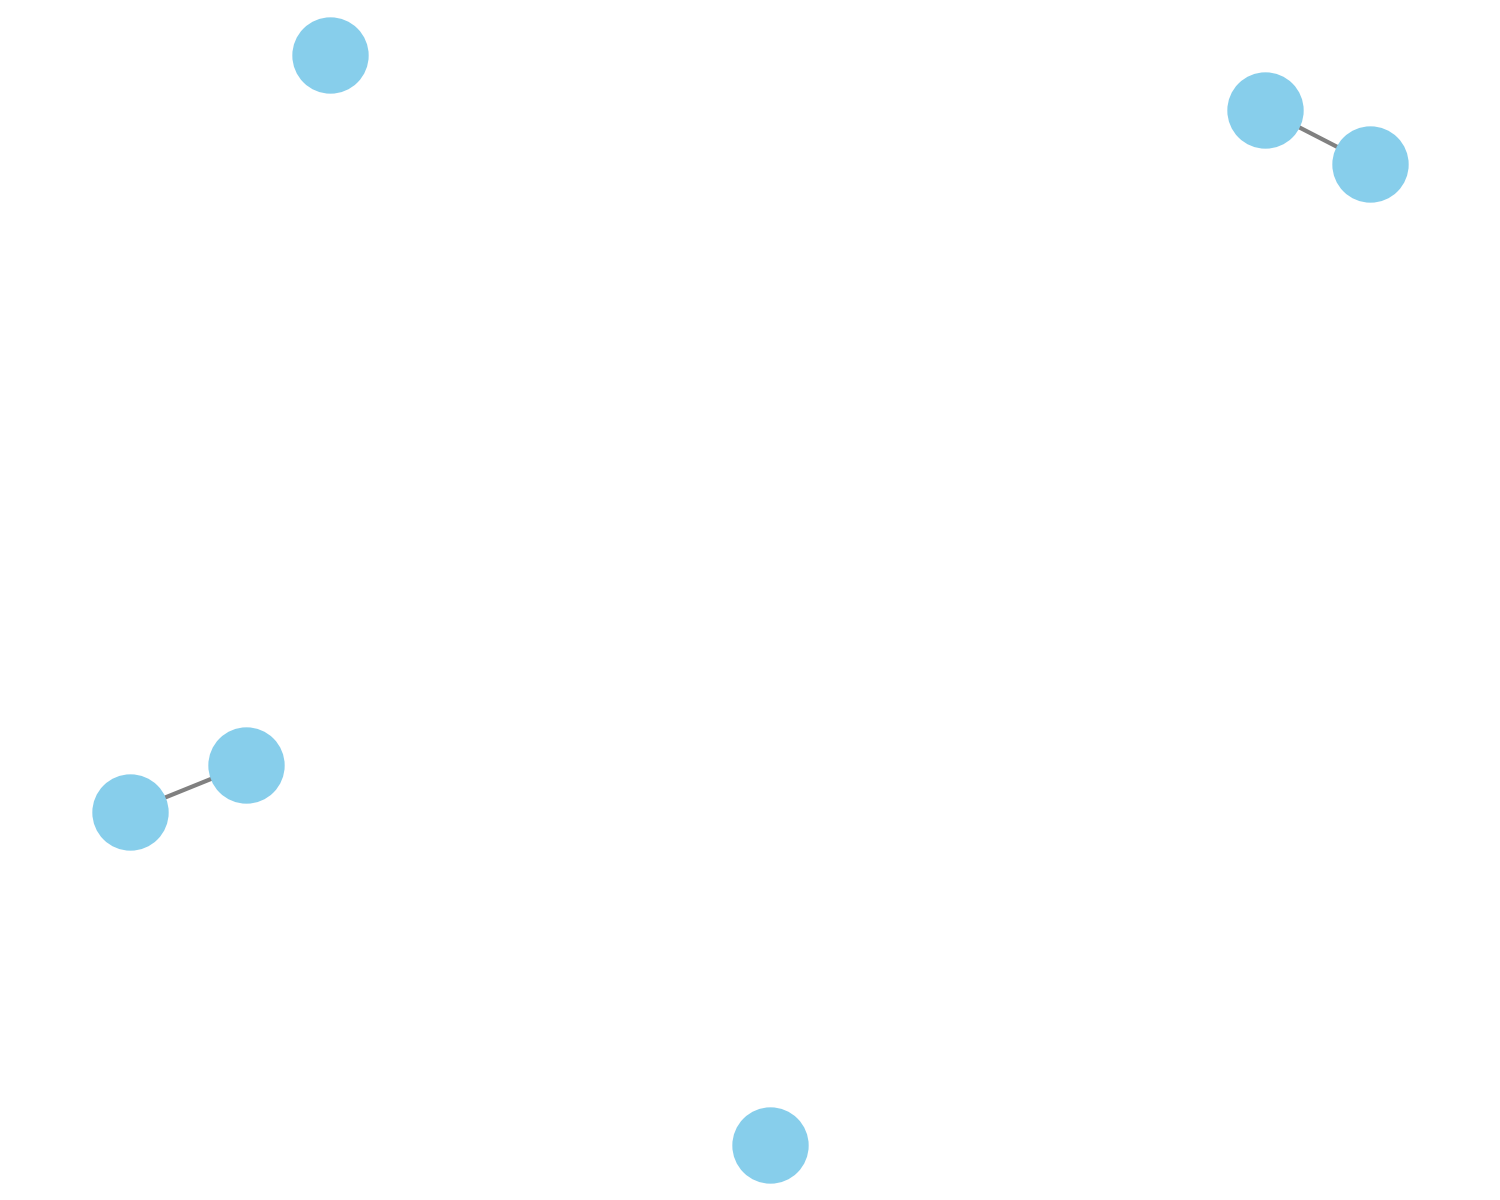
\includegraphics[width=0.75\textwidth]{figures/field_schematic.png}
    \caption{Timing alignment in field test protocol.}
\end{figure}

\section{Statistical Tests}
\subsection{Global EEG--Astro Data Correlation}
\textbf{Goal:} Check for non-random correlations between EEG datasets and cosmic/magnetic field data.
\textbf{Protocol:}
\begin{enumerate}
 \item Collect open EEG datasets and geomagnetic/astronomical time series.
 \item Apply preprocessing and time alignment.
 \item Compute correlation/coherence measures; assess significance.
\end{enumerate}
\textbf{Equipment:} Data sources, computing resources.
\begin{figure}[h]
    \centering
    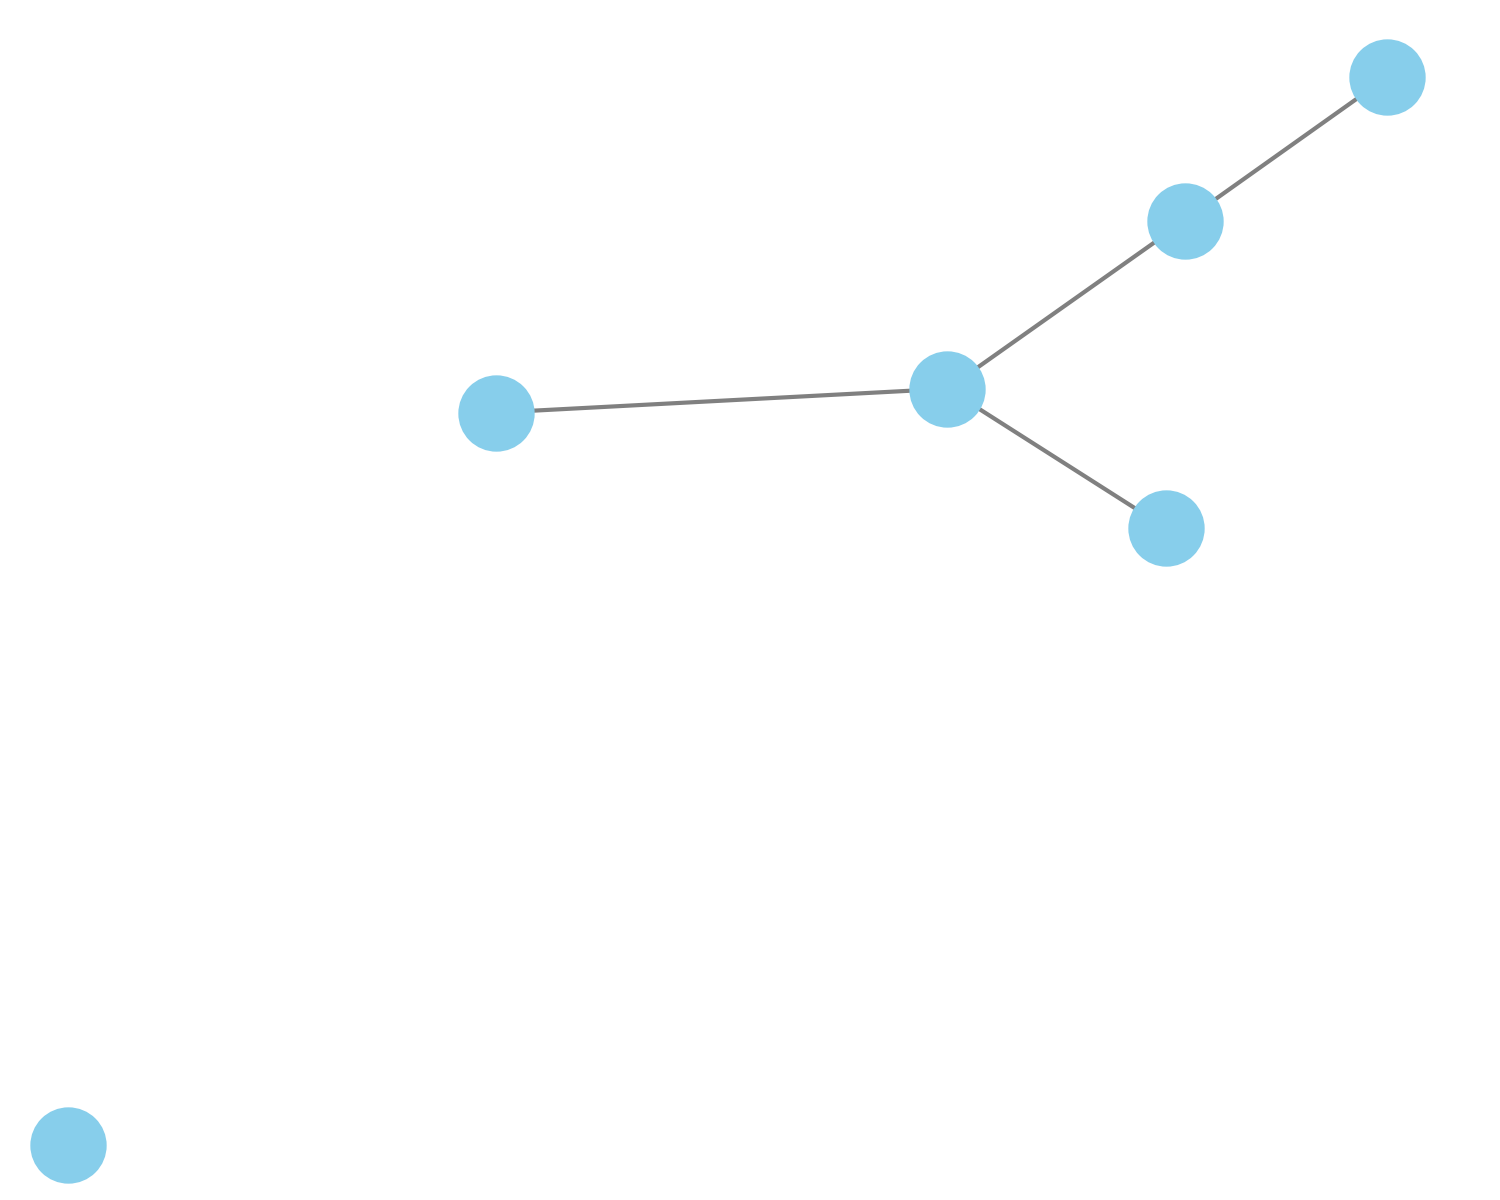
\includegraphics[width=0.75\textwidth]{figures/stats_schematic.png}
    \caption{Conceptual pipeline for statistical correlation analysis.}
\end{figure}

\end{document}
